\documentclass{article}

% Target journal: Molecular Phylogenetics and Evolution
%
% From author guidelines:
%
% Short communications of approximately 3000 words are also accepted. 
% These papers should contain no more than two figures, two tables, and thirty references. 
% A short abstract of fewer than 200 words is acceptable.


% Annotation/feedback commands
\newcommand*\rampal[1]{\textcolor{red}{\textbf{[RSE: #1]}}}
\newcommand*\richel[1]{\textcolor{orange}{\textbf{[RJCB: #1]}}}
\newcommand*\gio[1]{\textcolor{green}{\textbf{[GL: #1]}}}

% Bibliography
\usepackage{natbib}
\bibpunct{(}{)}{;}{a}{}{;}

\usepackage[english]{babel}

% Use 'It was found that something is something (Name 1234)' style
\setcitestyle{authoryear,open={},close={}}

% Affiliations
\usepackage{authblk}
\title{The error in Bayesian phylogenetic reconstruction when speciation co-occurs}

\author[1]{Giovanni Laudanno}
\author[1]{Rich\`el J.C. Bilderbeek}
\author[1]{Rampal S. Etienne}
\affil[1]{Groningen Institute for Evolutionary Life Sciences, University of Groningen, Groningen, The Netherlands}

% Use double spacing
\usepackage{setspace}
\doublespacing

\usepackage{pgf}
\usepackage{hyperref}
\usepackage{verbatim}
  
% Adds numbered lines
\usepackage{lineno}
\linenumbers

\hyphenation{
  BEAST
  Pa-ra-me-ter
  Drum-mond 
  Bayes-ian 
  Mr-Bayes 
  ap-proach-es 
  Rev-Bayes 
  cre-ate
  spe-ci-a-tion-com-ple-tion
  pro-trac-ted
 }

\begin{document}

\maketitle

%%%%%%%%%%%%%%%%%%%%%%%%%%%%%%%%%%%%%%%%%%%%%%%%%%%%%%%%%%%%%%%%%%%%%%%%%%%%%%%%%%%%%%
\begin{abstract}

  % From 'How to construct a Nature summary paragraph'

  % A short abstract of fewer than 200 words is acceptable.

  % One or two sentences providing a basic
  % introduction to the field,
  % comprehensible to a scientist in any discipline.
  

  % Two to three sentences of
  % more detailed background, comprehensible to
  % scientists in related disciplines.
  

  % One sentence clearly stating the general
  % problem being addressed by this particular
  % study.
  

  % One sentence summarising the main
  % result (with the words “here we show”
  % their equivalent).
  

  % Two or three sentences explaining what
  % the main result reveals in direct
  % comparison to what was thought to be the case
  % previously, or how the main result adds to
  % previous knowledge.

  % One or two sentences to put the results into a
  % more general context.


  % Two or three sentences to provide a
  % broader perspective, readily comprehensible
  % to a scientist in any discipline, may be included
  % in the first paragraph if the editor considers that the accessibility of the paper is significantly enhanced
  % by their inclusion. Under these circumstances, the length of the paragraph can be up to 300 words.
  % (The above example is 190 words without the final section, and 250 words with it).



\end{abstract}

{\bf Keywords:} computational biology, evolution, phylogenetics, Bayesian analysis, tree prior
%%%%%%%%%%%%%%%%%%%%%%%%%%%%%%%%%%%%%%%%%%%%%%%%%%%%%%%%%%%%%%%%%%%%%%%%%%%%%%%%%%%%%%
\gio{According to my fine graining approach we should at each step deepen every small section. At a certain level I think we can start to re-coarse-grain what we wrote to create the abstract.}
\richel{I enjoy this approach! Did some minor fine-graining}
\richel{Have you already looked up for a target journal? I know how a journal's constraints have helped me 
\gio{Honestly I have literally no idea how to select a good journal for this kind of article.}
in writing an article, for example, by having a maximum number of pictures}

%%%%%%%%%%%%%%%%%%%%%%%%%%%%%%%%%%%%%%%%%%%%%%%%%%%%%%%%%%%%%%%%%%%%%%%%%%%%%%%%%%%%%%
\section{Introduction}
\begin{itemize}

\item There are many contemporary tools that provide the possibility to infer a phylogeny from genetic data (DNA, RNA, proteins). A popular Bayesian
phylogenetic tool is called BEAST (\cite{beast}) and its cousin BEAST2 (\cite{beast2}).

\item BEAST is very flexible, providing the user with the option to set up all possible phylogenetic priors (e.g. site/clock/speciation model).

%Current limits in current tools.
\item However, currently available priors can be not suitable to analyze some specific datasets. 
%With this work we aim to test whether or not the implementation of a new prior model is beneficial to study a specific kind of diversification process.

\item BEAST2 gives us the possibility to introduce new tree priors to infer phylogenies based on different assumptions on how the speciation process
takes place.

\item One of such speciation processes is the multiple birth hypothesis,
a new model (described below) and thus currently absent in BEAST.

\item The Multiple birth hypothesis can be useful to explain a phenomenon that has always puzzled evolutionary biologists: what are the drivers of the diversification processes for those phylogenies that show an impressive amount of speciation events in relatively short times? 
The (constant-rate) birth-death (BD) model embodies the common assumption that 
only a single speciation event can occur at any given time.
The multiple-birth-death (MBD) model 
\richel{I feel MBSD (Multiple Birth Single Death) may be a better name: extinctions are still one at a time}
\gio{I always had the same doubt. The problem is that a good name should be, at the same time, both descriptive and short. I'll think about that.}
relaxes this assumption, allowing events in which 
large-scale environmental changes lead to a great number of species 
in relatively short time intervals. Such a hypothesis may be a better fit to describe the burst in in systems like cichlid fish diversification in the 
African Great Lakes: Malawi, Tanganyika and Victoria (\cite{janzen2016}, \cite{janzen2017}).

\item However, it may be that current BD tree priors are good enough at detecting such events, with a (preferred) lower level of complexity. If this is the case one should always be more keen to adopt the simplest model.

\item Here we present our study with the aim of exploring when using a more complex MBD tree prior is warranted.

\end{itemize}
%%%%%%%%%%%%%%%%%%%%%%%%%%%%%%%%%%%%%%%%%%%%%%%%%%%%%%%%%%%%%%%%%%%%%%%%%%%%%%%%%%%%%%

%%%%%%%%%%%%%%%%%%%%%%%%%%%%%%%%%%%%%%%%%%%%%%%%%%%%%%%%%%%%%%%%%%%%%%%%%%%%%%%%%%%%%%
\section{Methods}

\subsection{Model}
\begin{itemize}

\item Current phylogenetic tools assume that only a single speciation event can occur at any given time.
While this assumption is useful to construct a wide variety of successful 
models (e.g \cite{Maddison2007biSSE}, \cite{Valente2015}, \cite{etienne2012diversity}, \cite{etienne2014estimating}),
they disallow for environmental changes that trigger speciations in multiple clades at a same point in time. 

\item The (constant-rate) birth-death (BD) model embodies the common assumption that 
only a single speciation event can occur at any given time.
The multiple-birth-death (MBD) model relaxes this assumption, allowing events in which 
large-scale environmental changes lead to a great number of species 
in relatively short time intervals. Such hypothesis can be useful to describe, for example, 
systems like cichlid fish diversification in the 
African Great Lakes: Malawi, Tanganyika and Victoria (\cite{janzen2016}, \cite{janzen2017}).

\item In the MBD model, parameters $\lambda$ and $\mu$ correspond, respectively, 
to the common per-species speciation and extinction rates present also in the standard BD model. 
Additionally, MBD relies on two additional parameters. Parameter $\nu$ is the rate at which an environmental change is triggered.
When such event is triggered, all species present in the phylogeny at that moment
have a probability $q$ to speciate at that time, which is 
independent on $\lambda$. 

\item It is also possible to write down a likelihood function for such processes as in \cite{mbd}.
    
\end{itemize}

\subsection{Simulations}
\begin{itemize}

\item To prove our hypothesis we simulate two twin datasets. All the simulations are produced in continuous time, using the Doob-Gillespie algorithm. 

\item We start simulating $N_{S} = 1000$ \richel{I will measure the number of trees we'll be able to simulate within a short enough time, when the experiment is set up} MBD trees. From each MBD tree, a DNA sequence alignment is simulated. For each sequence alignment we then perform a Bayesian analysis to recover a posterior distribution of trees, each composed of $N_{P}$ phylogenies. Such analysis is performed using 
the 'pirouette' package (\cite{pirouette}) to call the BEAST2 tool 
suite from R. We let the Bayesian analysis assume a BD prior, to investigate
the error this inference makes due to this.

\item For each tree 
generated under the MBD model we aim to generate a "twin" tree under the BD model in order to perform a fair comparison. 
We want trees from the two models to contain the same amount of information, 
i.e. the same (expected) number of DNA mutations. %option 1
%i.e. the same number of taxa at the present. %option 2
To obtain these twin trees, 
\richel{
  I suggest to first start with the equal number of taxa,
  and the calculation of the speciation rates first.
}
\gio{@richel: both assumptions seem to make sense to me. If possible I would run both and see which one performs better. For now let's stick to option 1 in the manuscript.}
we impose
that the expected number of mutations in an MBD tree, $m_{MBD}$ equals
the expected number of mutations in a BD tree, $m_{BD}$:

\begin{equation}
m_{MBD} = m_{BD} \label{m equivalence}
\end{equation} 

We first generate a set of MBD trees. For each of them we can measure the amount of mutations $m_{MBD}$.

\gio{I think this should definitely go to the methods}
\richel{I put it there for use, hopefully at a spot you liked :-)}

The expected number of mutations $m$ of a phylogeny 
\richel{
  I think 'expected number of mutations' would be more correct.
  Do you agree?
}
\gio{I don't agree. It is expected if you use an expected number of species over time. If you have the correct $n(t)$ in principle you should be able to get the exact number of mutations.}
with crown age $-T$ (with $T>0$) in fact is given by
\richel{
  above stood 'crown age -T'. 
  I feel that a crown age is a positive number,
  but I know you have had a good reason.
  Perhaps better would be to write something explicit like:
  t\_now - t\_crown = T.
  Looking forward for a better suggestion than mine :-)
}
\gio{We can specify that the crown age is $-T$ where $T$ is a positive number (which should be already clear, I guess, if we report it as $-T$). In my opinion this makes everything nicer when we have to write down the integral which should, in principle, be $\int_{-T}^{0} f(t-(-T))$ but using integral properties can be rewritten as $\int_{0}^{T} f(t)$. Having a definite integral starting from $0$ always looks better ^^.}

\begin{equation}
m = L \cdot \rho \cdot \int_{0}^{T} n(t)\ dt \label{m calculation}
\end{equation}

where $L$ is the number of DNA nucleotides, 
$\rho$ is the per-site per-species mutation rate and
$n(t)$ the number of species at each time.

%It can be easily seen considering that $\rho$ is the number of mutations
%per unit time per site. For this reason it's needed to multiply by
%time and number of sites. 
\gio{This feels kind of a repetitions of what we wrote before the formula. I comment it. We can think of reinsert it afterwards, if needed (see comment above).}
\richel{
  I suggest to remove such commented-out lines. 
  Although I sometimes get attached to my sentences,
  they clog up the document by non-info and 
  I usually delete them anyways in the end.
  I cannot remember ever regretting this (would I, 
  I could find it in the git history).
  Would you agree?
}
\gio{Agree. Remove them. CLOSED}

Since we cannot know $n_{BD}(t)$ before running simulations
we need to replace it with a proxy. 
For this reason we will use the average number of
species in time according to the BD model. 
It's well known that this is equal to \gio{insert proper citation}
\richel{
  I see you use angle bracket as a notation for the expected
  value. I usually see 'E(x)' as the expected value for 'x',
  and this is used at the beloved https://en.wikipedia.org/wiki/Expected\_value.
  What are the reasons you prefer the notation with the angle brackets?  
}
\gio{Because the capital E is inelegant, plebeian and boor. And we want to be classy, don't we? :D}

\begin{equation}
    <n_{BD}>(t) = n_{0} \cdot e^{(\mu_{BD} - \lambda_{BD})t} \label{BD average n}
\end{equation}

where $n_{0} = n_{BD}(-T) = n_{MBD}(-T)$ is the initial number of species at the crown age.
From \ref{m equivalence}, \ref{m calculation} and \ref{BD average n} follows:

\begin{equation}
m_{MBD} = L \cdot \rho \cdot \int_{0}^{T} <n_{BD}>(t)\ dt \\
= L \cdot \rho \cdot n_{0} \cdot \left[ \frac{e^{(\mu_{BD} - \lambda_{BD})T} - 1}{\mu_{BD} - \lambda_{BD}} \right]
\end{equation}

If we set $\mu_{BD} = \mu_{MBD}$ and reverse this relation we can extrapolate the value of $\lambda_{BD}$ to use to generate BD trees.

\richel{I suggest $n_{BD} = n_{MBD}$ and only 
change $\rho_{BD}$ to reach $<m_{MBD}> = <m_{BD}>$}
\gio{@Richel: Don't you think it might make more sense to set $\mu_{BD} = \mu_{MBD}$? What changes in the two model is the way we use to generate new species, not the way to remove them. Maybe one thing that's possible to do would be to make $\lambda_{BD}$ a function of time, a bit like Théo is doing in his comparison between DD and TD4 (which, by the way, seem to yield very different results). In case you are wondering the theory can be found in Caesar's master thesis.}
\richel{
  I fully agree to use the same extinction rates!
  The 'mu' used in the context of mutations (now 'rho') messed me up.
  I hope this is clear now. To recap: 
  (1) calculate the speciation rate of the twin tree as you wrote down excellently,
  (2) simulate a twin tree with same number of taxa,
  (3) calculate the mutation rates of the trees, 
    so their alignments contain as much information
}

\gio{My doubt is if we need to use $m_{MBD}$ for the single tree or the same
quantity averaged on the full MBD dataset $<m_{MBD}>$.
Do you think is better to use the
individual $m_{MBD}$ for each tree or the average across the whole
dataset?}
\richel{
  I think a per-tree calculation of the mutation rates 
  is the best we can do. As there was some noise between us above,
  I think the iteration after the next will allow us to get a better
  idea about this
}
\gio{I am still very debated about this. I actually would like to ask also Rampal's opinion.
}
\begin{figure}[!htbp]
  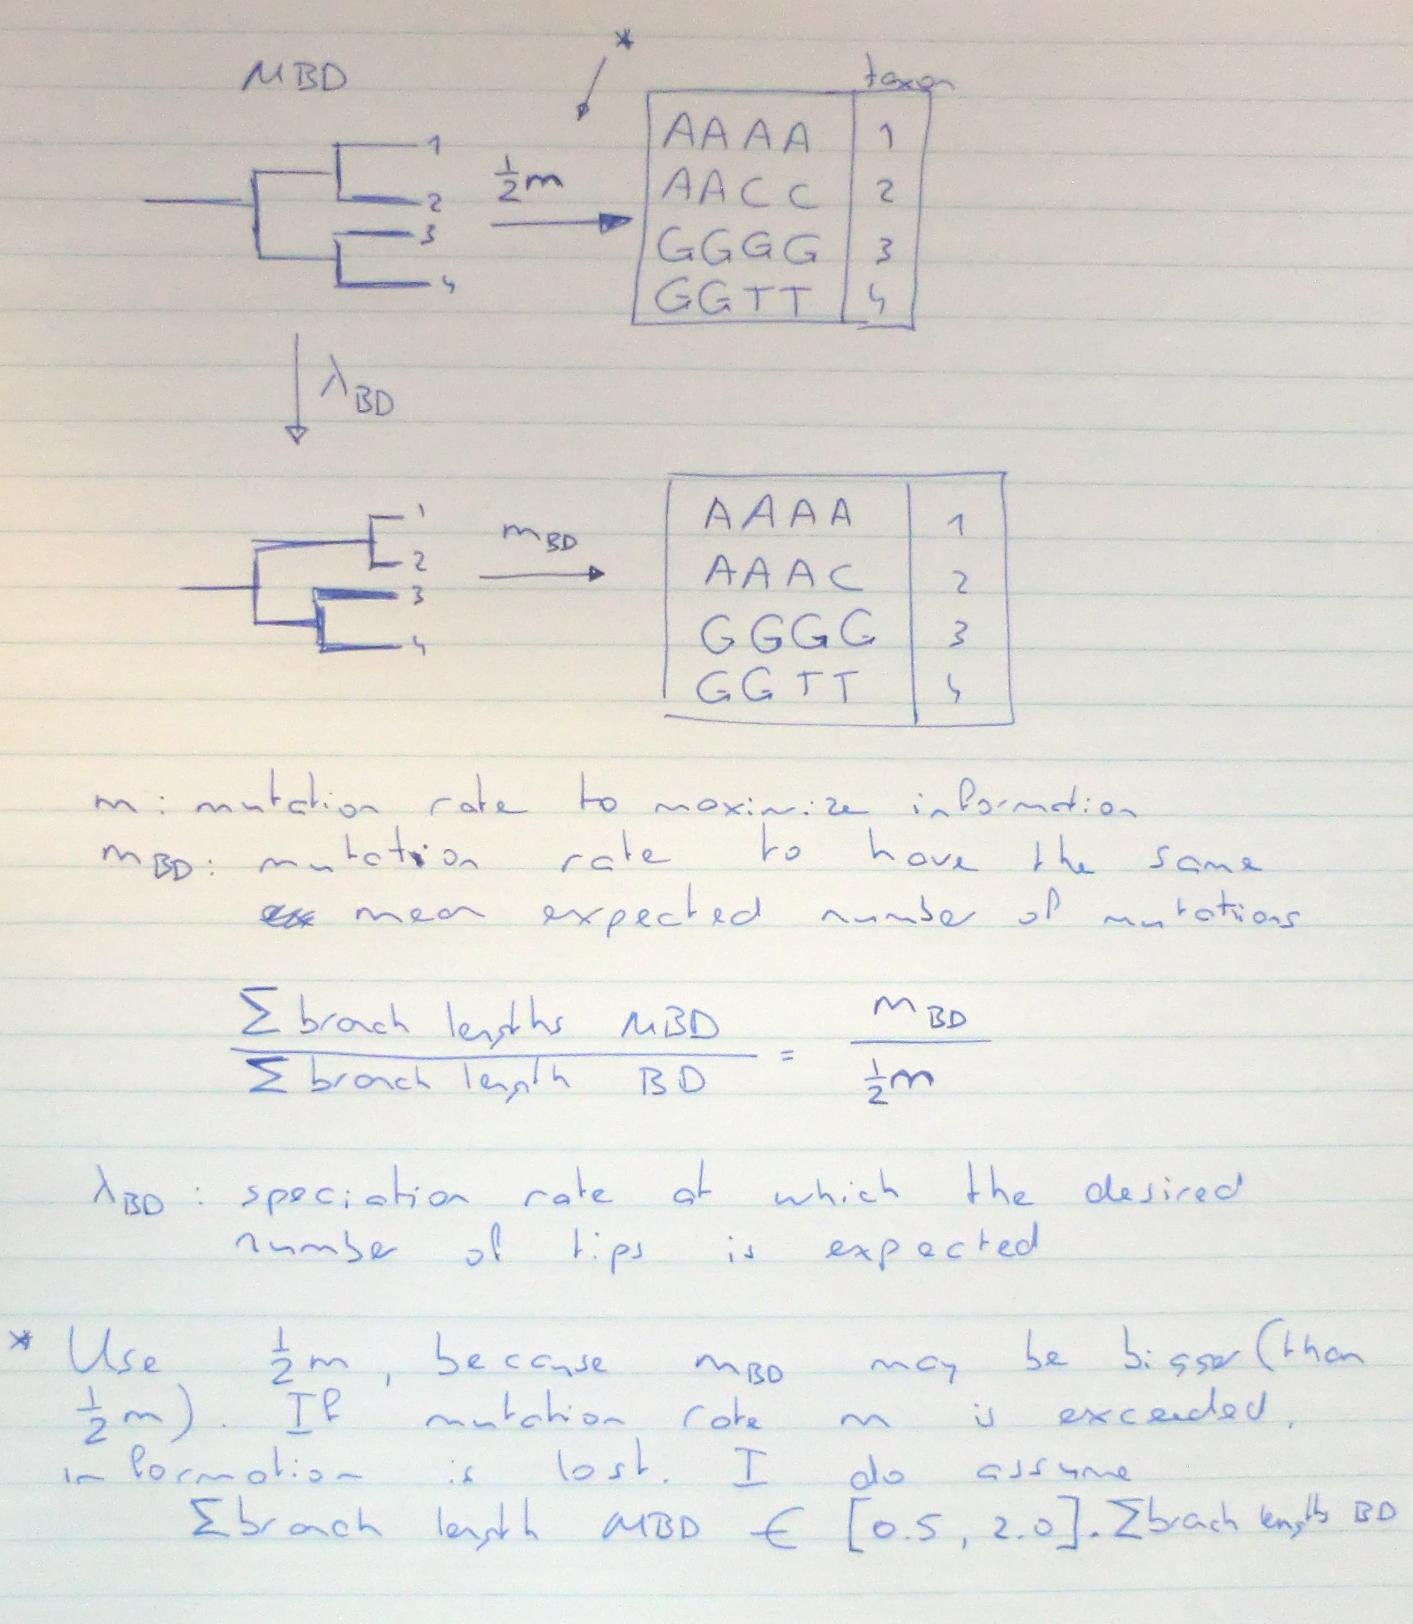
\includegraphics[width=\textwidth]{mbd.jpg}
  \caption{
    How to create twin trees and alignments. From a focal MBD tree, a twin tree is produced as 
    such: (1) estimate the $\lambda_{BD}$ to get the same expected number of tips, (2) simulate a BD tree with that amount of tips (discard trees with different number of tips), (3) estimate a mutation rate to get an alignment with the same expected number of mutations, (4) simulate alignments with that amount of mutations (discard those that don't, the picture shows an alignment that should be discarded) 
  }
\end{figure}

\item We explained how we set the parameters for each twin BD tree. Using this rules we generate a BD dataset. We repeat the analysis, producing alignments for each tree and subsequently using BEAST to produce a posterior for each of them.

\subsection{Model selection}

\item So far we have simulated two datasets of trees under the two models: $\{T_{i}^{BD}\}_{i=1}^{N_{S}}$ and $\{T_{i}^{MBD}\}_{i=1}^{N_{S}}$.
We used them to generate a dataset of alignments for each model: $\{X^{BD}_{i}\}_{i=1}^{N_{S}}$ and $\{X^{MBD}_{i}\}_{i=1}^{N_{S}}$. From each dataset we produced a posterior distribution from a BD prior: 
$P_{i}(\theta | X^{BD}_{i}, BD)$ and $P_{i}(\theta | X^{MBD}_{i}, BD)$.
\gio{1) We might want to rename the models, e.g. BD = (0) and MBD = (1). These names with capital letters are too big and ugly;
2) Writing down things to tidy up manuscript and thoughts I just realized that actually the "model" is the same for the two posteriors. In fact with the word "model" Maturana et al. refer to the prior used (see eq. 1, $\pi(\theta | M)$). In such case are we sure we can actually use the Bayes factor for model selection?}
%Now we have two datasets  of posteriors to compare, one for the BD model and one for the MBD model.

\subsubsection{Option 1: nLTT statistics}
\item To compare the results for the two models we measure the inference error using the nLTT statistic between known/true tree and posterior/inferred trees (\cite{nltt}). To obtain such statistics the procedure is the following:

- From each tree $T_{i,j}^{M}$ (with $j=1,...,N_{S}$) belonging to the posterior $P_{i}(\theta | X^{M}_{i}, BD)$ and relative to the model $M$, we extrapolate the lineage-through-time (LTT), in other words we measure the number of species as a function of time $n_{i,j}(t)$. To allow a comparison we normalize dividing by the maximum number of species of each tree, i.e. the number of tips at the present $N_{i,j}(t)=\frac{n_{i,j}(t)}{n^{max}_{i,j}}$. We then define the nLTT measure as

$nLTT_{i,j} = \int_{0}^{T} \abs{N_{i,j}(t) - N_{T_{i}}} dt$

\gio{I am running out of letters :(}
\richel{
  I would love to describe this more concrete. For example, when do
  we say something has an effect? If we avoid making such judgements,
  how will we visualize?
}

\subsubsection{Option 2: Bayes Factor (BF)}

\richel{I removed the Bayes factor text. It is useful when letting BEAST2
pick more/overly complex models and see if that more complex model fits the
data better (penalized by its increased complexity, similar to the AIC). It has
its uses, but I am unsure if we already want to discuss this now
or first focus on the proper tree twinning}
\gio{But after we describe the tree twinning we will have to describe the method we use for model selection anyways. BF and nLTT are mutually exclusive choices, right?}
\gio{The point is: what method do we choose? According to the choice we have to describe that. I'd also like to know Rampal's opinion on that. In principle I like more the BF method cause it looks more solid while the nLTT looks a bit like the last resort to me.}



\end{itemize}
%%%%%%%%%%%%%%%%%%%%%%%%%%%%%%%%%%%%%%%%%%%%%%%%%%%%%%%%%%%%%%%%%%%%%%%%%%%%%%%%%%%%%%

%%%%%%%%%%%%%%%%%%%%%%%%%%%%%%%%%%%%%%%%%%%%%%%%%%%%%%%%%%%%%%%%%%%%%%%%%%%%%%%%%%%%%%
\section{Results}
\begin{itemize}

\item
\richel{
  I guess you know I am a fan of the Open Science Framework,
  in which you first register you work before you do the experiment
  (note: I will do some small pilots to estimate the complete time
  of the experiment). I think it is the proper and superior science,
  which helps us against writing down bullshit stories after having
  obtained the results (e.g. 'We expected A and indeed found it!').
  It also helps me structure my work: first think
  deeply about the experiment, then do it (instead of the mixing
  up the two phases). What are your thoughts on that?
}
\gio{I agree on the principle but I don't fully agree on the open science procedure. Sometimes you do find something good while you're looking for something else. That happened many times in the history of science. This doesn't necessarily implies that we will end up p-hacking the results. I think we need to be open to new findings that might be not forecasted by our hypothesis. I think this is the good way to do science: be critical with our results but not imposing that reality will follow the theory.}
\item

\end{itemize}
%%%%%%%%%%%%%%%%%%%%%%%%%%%%%%%%%%%%%%%%%%%%%%%%%%%%%%%%%%%%%%%%%%%%%%%%%%%%%%%%%%%%%%

%%%%%%%%%%%%%%%%%%%%%%%%%%%%%%%%%%%%%%%%%%%%%%%%%%%%%%%%%%%%%%%%%%%%%%%%%%%%%%%%%%%%%%
% Bibliography % MEE style
\bibliographystyle{mee}
\bibliography{article}
%%%%%%%%%%%%%%%%%%%%%%%%%%%%%%%%%%%%%%%%%%%%%%%%%%%%%%%%%%%%%%%%%%%%%%%%%%%%%%%%%%%%%%

%%%%%%%%%%%%%%%%%%%%%%%%%%%%%%%%%%%%%%%%%%%%%%%%%%%%%%%%%%%%%%%%%%%%%%%%%%%%%%%%%%%%%%
\appendix


%%%%%%%%%%%%%%%%%%%%%%%%%%%%%%%%%%%%%%%%%%%%%%%%%%%%%%%%%%%%%%%%%%%%%%%%%%%%%%%%%%%%%%


\end{document}